\section{Spinpräzession im Erdmagnetfeld}
\subsection{Durchführung}
Die Bestimmung der Spinpräzession im vertikalen Erdmagnetfeld erfolgt folgendermaßen:
Das \textlambda/4-Plättchen im Strahlengang erzeugt zirkular polarisiertes Licht,
durch das die Rubidiumatome im Magnetfeld optisch gepumpt werden.
Das Magnetfeld wird von Spule~5 erzeugt, ihre Stromversorgung erfolgt vom \emph{instec function~generator}.
Der Funktionsgenerator erzeugt ein Rechtecksignal mit einer Spitze-zu-Spitze-Amplitude von 260\,mV und
einem Offset von 130\,mV, sodass das Magnetfeld periodisch an- und ausgeschaltet wird.
Um das Erdmagnetfeld in Strahlrichtung zu kompensieren,
wird ein Strom von $I_1$=17\,mA durch Spule~1 geschickt.
Die Temperatur des Peltierelements beträgt bei den Messungen 33.9$^\circ$C.
Es werden zuerst zwei Messreihen durchgeführt, um die beiden Rubidiumisotope zu untersuchen:
Mit 63.7\,mA Laserstrom (Pumpen von \rb{85}) und mit 64.1\,mA (\rb{87}).
Während einer Messreihe wird der Strom durch Spule~4 zwischen 0\,mA und 100\,mA variiert und
so die Vertikalkomponente des Magnetfelds beeinflusst
(eine Kompensation des vertikalen Erdmagnetfeldes findet bei ca. 90\,mA statt).
Das Transmissionssignal der Messzelle wird mit dem Oszilloskop gemessen und
es findet eine Heizung mit dem Föhn statt.

Nach Durchführung der ersten beiden Messungen wurde festgestellt,
dass mit der Variation des Stroms durch Spule~4 keine vollständige Kompensation des Magnetfelds möglich ist.
(Eine vollständige Kompensation würde sich darin zeigen,
dass die Frequenz der Spinpräzession sehr groß wird und keine Präzession mehr messbar ist).
Dies wurde auf die Anwesenheit der Horizontalkomponente des Erdmagnetfeldes
senkrecht zum Strahlengang zurückgeführt, da der Messaufbau nicht parallel zum Horizontalanteil des
Erdmagnetfelds ausgerichtet ist und durch Spule~1 nur ein Magnetfeld parallel zum Strahlengang kompensiert wird.

Aus dem Anteil des Magnetfelds, das bei den ersten beiden Messreihen nicht kompensierbar war
(dieser Anteil wurde mit einem Modell bestimmt, das an die Messdaten angepasst wurde),
konnte die Abweichung des Messaufbaus von der Nordausrichtung vorhergesagt werden.
Der Messaufbau wurde um den so bestimmten Winkel gedreht und eine weitere Messreihe an \rb{85} durchgeführt,
um eine vollständige Magnetfeldkompensation und ein Verschwinden der Spinpräzession zu erreichen.
Zusätzlich wurde bei einem Strom von 90\,mA durch Spule~4 die Winkelabhängigkeit der Präzessionsfrequenz untersucht.


\subsection{Auswertung}
\begin{figure}[H]
\begin{center}
  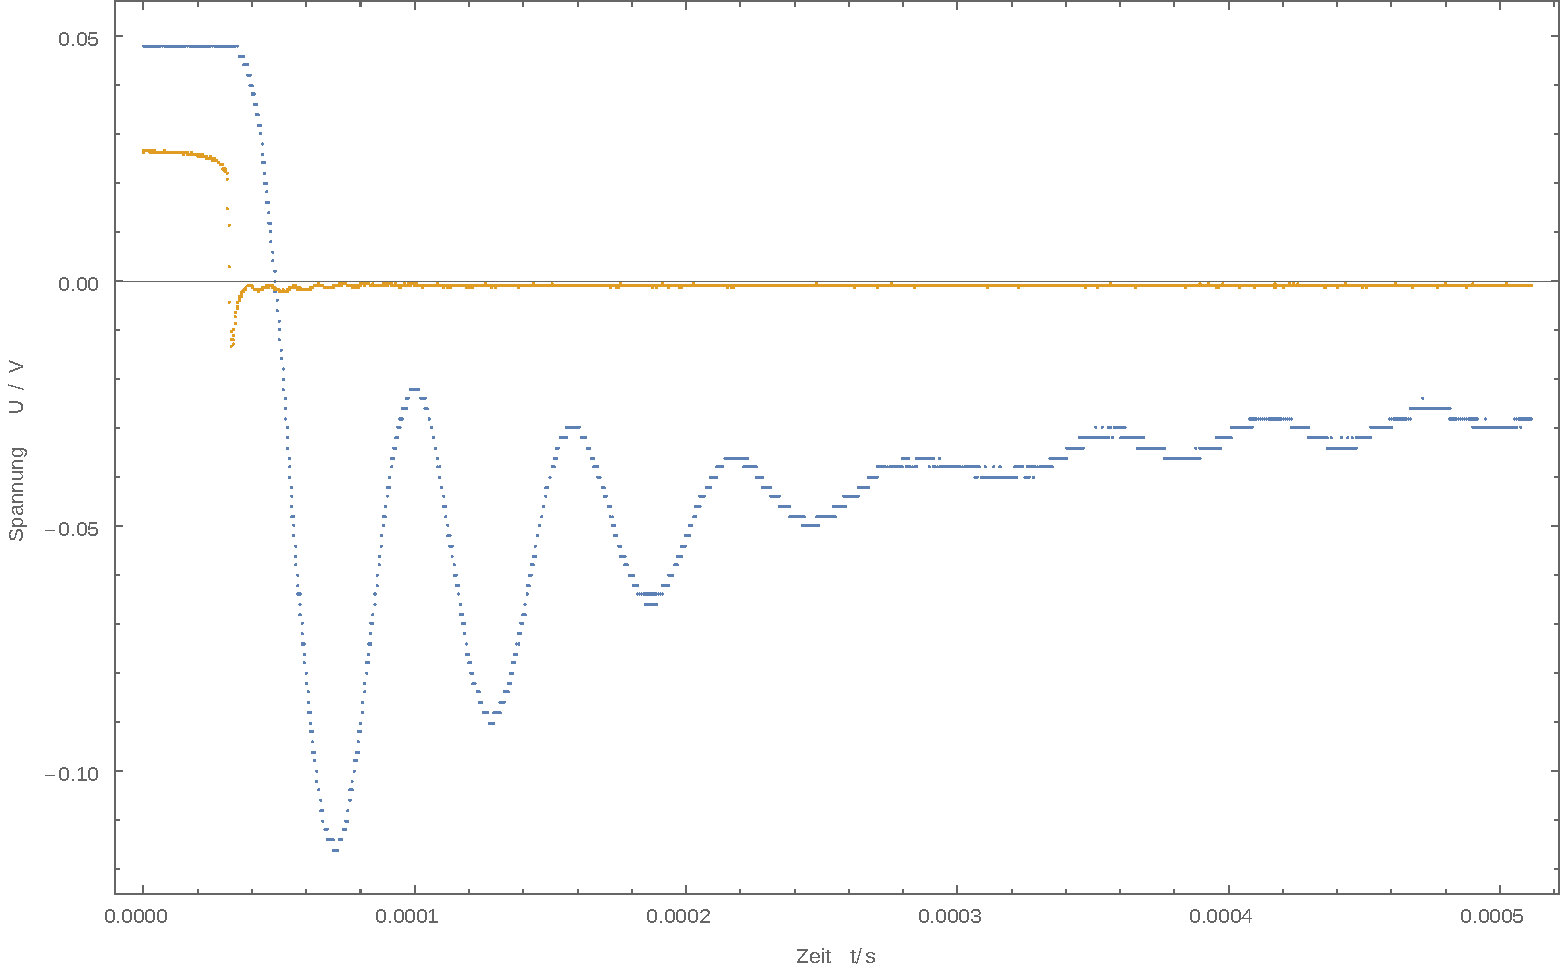
\includegraphics[width=\textwidth]{../img/part4/dummyExampleSpinpr.pdf}
  \caption{Spinpräzession des Rubidiumensembles, sichtbar in der Transmissionsoszillation der Messzelle.}
  \label{img:spp:expl}
\end{center}
\end{figure} 

\autoref{img:spp:expl} zeigt eines der gemessen Spinpräzessionssignale.
Zur Bestimmung der Präzessionsperiodendauer $T$ wurden die Zeitkoordinaten $t_1$ und $t_2$
von zwei möglichst weit voneinander entfernten Maxima per Hand abgelesen und durch
die Zahl $n$ der dazwischenliegenden Perioden geteilt:
\begin{equation}
  T=\frac{t_2-t_1}{n}=f^{-1}, \qquad s_f = n \frac{\sqrt{s_{t_2}^2 + s_{t_1}^2}}{ \left( t_2 -t_1 \right)^2 }
\end{equation}
Die Präzessionsfrequenz ist $f$ bezeichnet.
Der relative Fehler auf die abgelesenen Zeiten wurde abgeschätzt auf $\frac{s_{t_i}}{t_i}=0.01$,
$n$ ist nicht fehlerbehaftet.

Aus dem Strom durch Spule~4 wurde mit \autoref{tab:inductorItoB} das erzeugte vertikale Magnetfeld
$B_\text{S,v}$ berechnet. Der Fehler auf den Strom beträgt $s_{I_4}=1$\,mA.

Die Abhängigkeit der Präzessionsfrequenz $f$ vom zusätzlichen Vertikalfeld $B_\text{S,v}$ ist auf
\autoref{img:spp:SPPRb85} gezeigt.
Ein erster Fit erfolgt mit
\begin{equation}
  f_1(B_\text{S,v})=\alpha \cdot |B_\text{E,v}-B_\text{S,v}| \ \, ,
\end{equation}
wobei $B_\text{E,v}$ die Vertikalkomponente des Erdmagnetfelds bezeichnet und
$\alpha_1$ eine Proportionalitätskonstante.
Es ist deutlich erkennbar, dass das lineare Modell die Messwerte nur beschreiben kann,
wenn sich die Richtung des effektiven Vertikalfeldes
$B_\text{E,v} \text{\,-\,} B_\text{S,v}$ in der Messreihe nicht umdreht.

\begin{figure}[H]
\begin{center}
  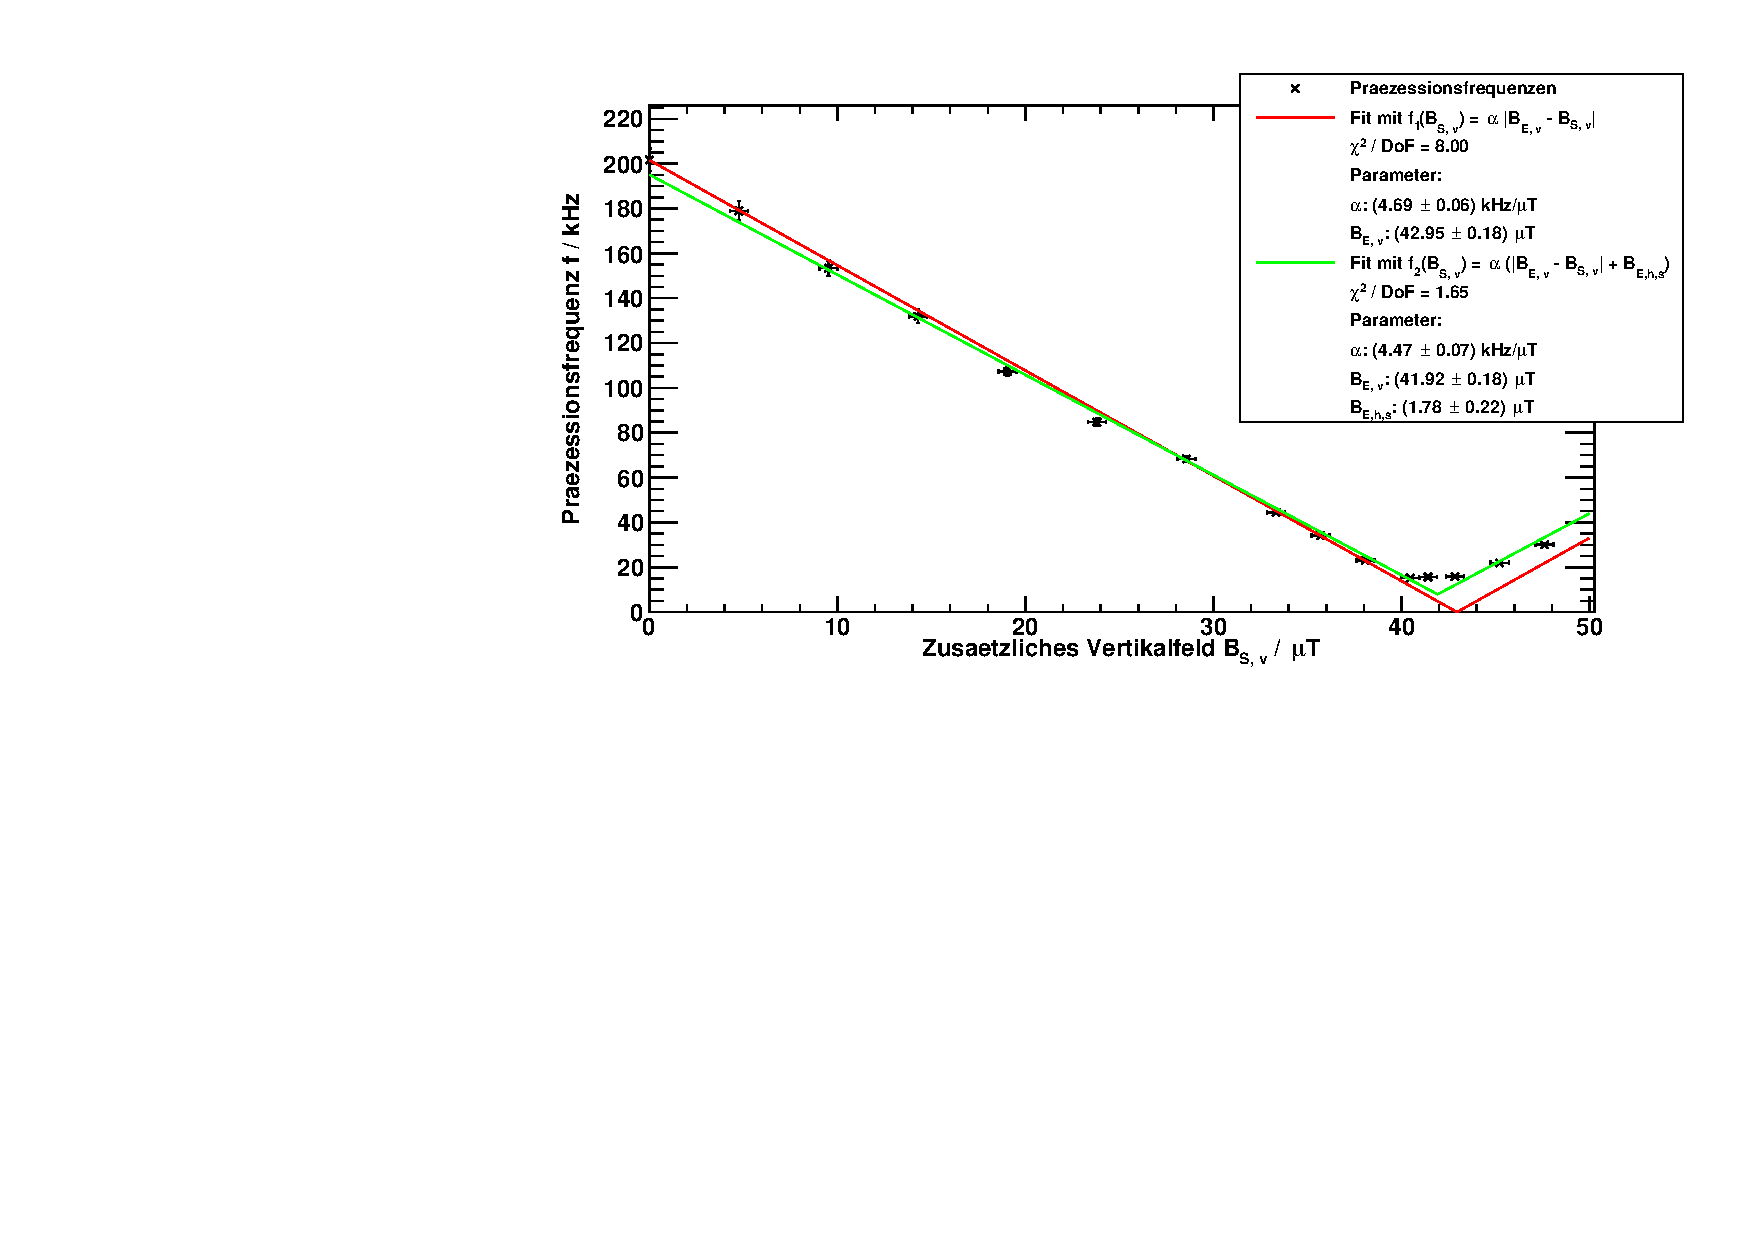
\includegraphics[width=\textwidth]{../img/part4/Rb85.pdf}
  \caption{Spinpräzessionsfrequenz $f$ von \rb{85} in Abhängigkeit
  vom zusätzlichen vertikalen Magnetfeld $B_\text{S,v}$, das dem Erdmagnetfeld überlagert ist.
  Der Fit erfolgt mit einem einfachen Modell sowie unter Berücksichtigung des
  nichtkompensierten Erdmagnetfelds~$B_\text{E,h,s}$.}
  \label{img:spp:SPPRb85}
\end{center}
\end{figure} 

Aus diesem Grund wird ein modifiziertes Modell verwendet, das der Tatsache Rechnung trägt,
dass der Horizontalanteil des Erdmagnetfelds senkrecht zum Strahl $B_\text{E,h,s}$
während der Messung unkompensiert bleibt:
\begin{equation}
  f_2(B_\text{S,v})=\alpha \cdot (|B_\text{E,v}-B_\text{S,v}| + B_\text{E,h,s}) \ \, .
\end{equation}
Dieses Modell eignet sich zur Beschreibung der Messdaten.

Die Auswertung erfolgt analog für das Isotop \rb{87} (\autoref{img:spp:SPPRb87}).
In \autoref{tab:spp:fitres} sind die Ergebnisse der aller vier Fits aufgeführt.

\begin{figure}[H]
\begin{center}
  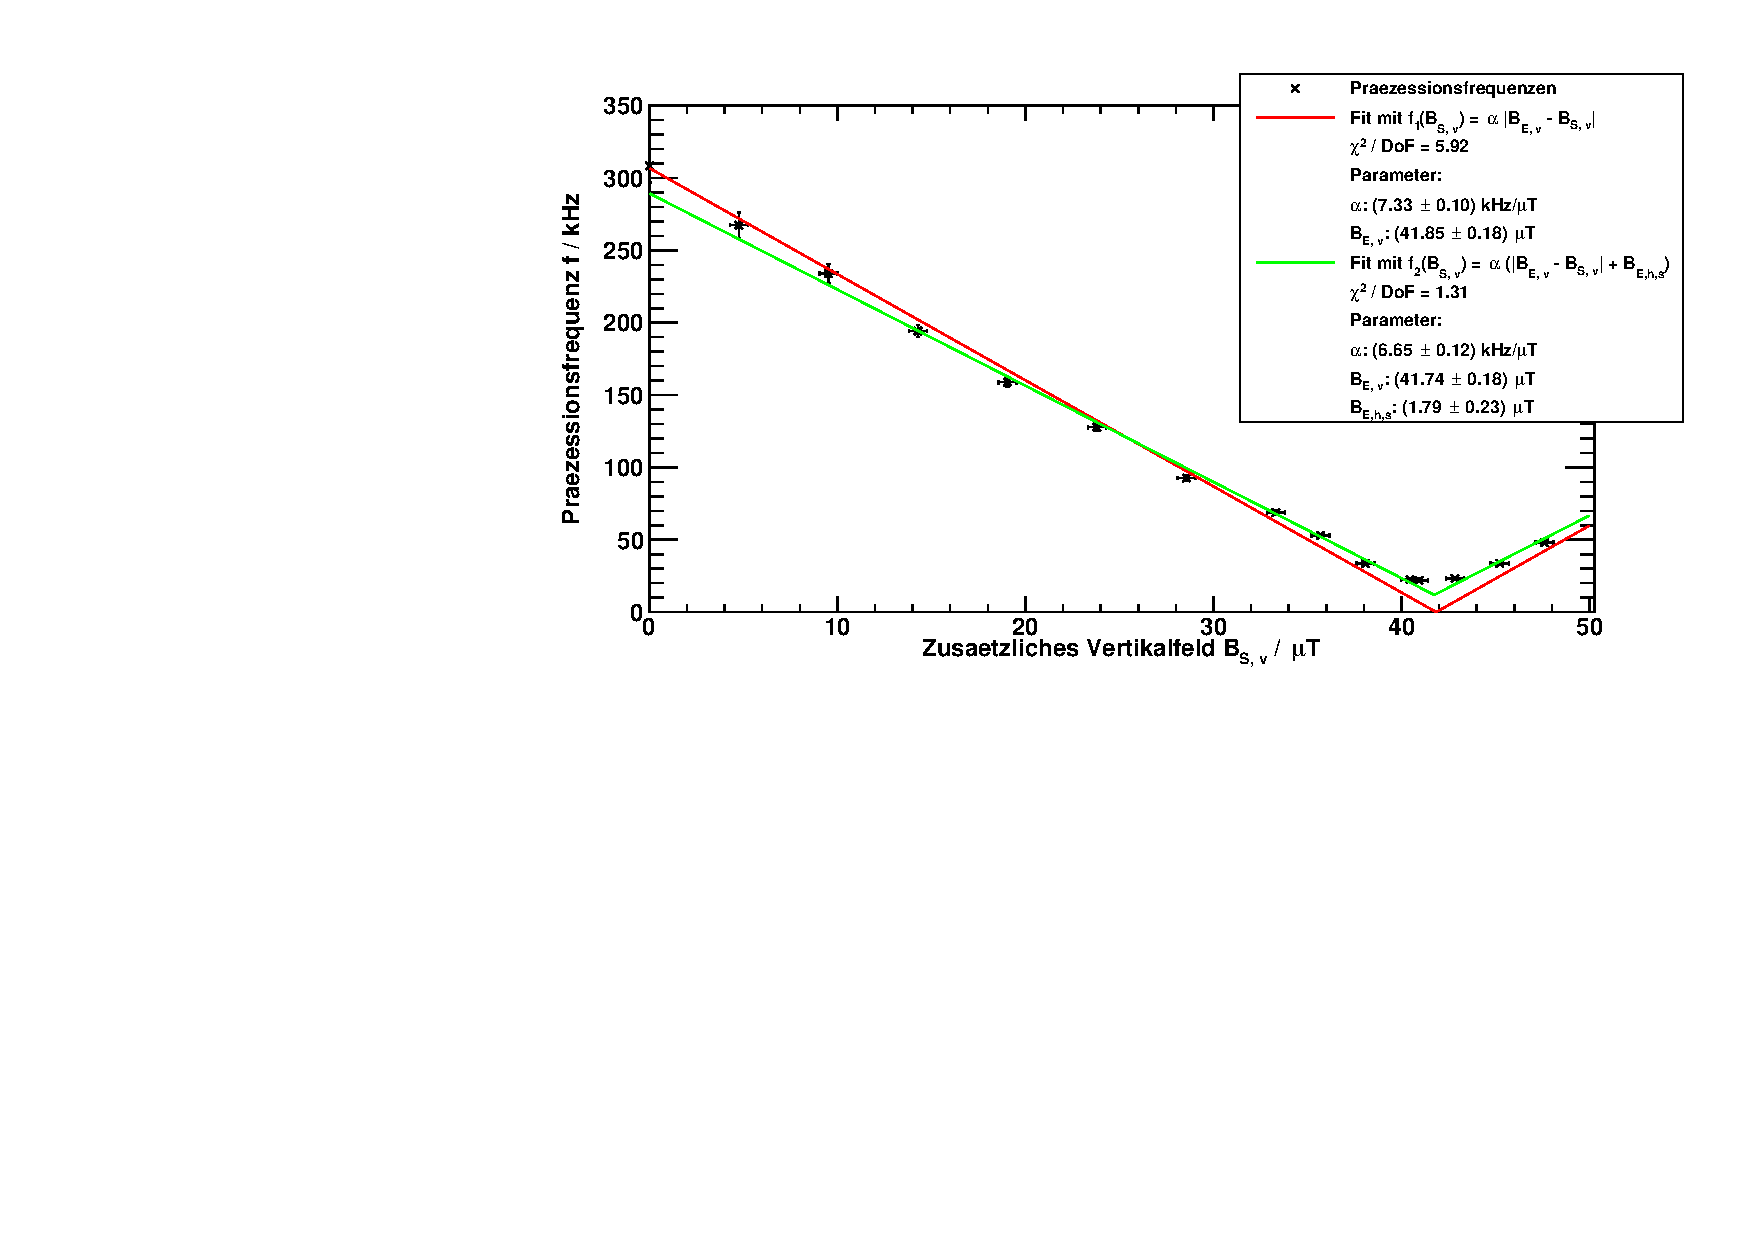
\includegraphics[width=\textwidth]{../img/part4/Rb87.pdf}
  \caption{Spinpräzessionsfrequenz $f$ von \rb{87} in Abhängigkeit
  vom zusätzlichen vertikalen Magnetfeld $B_\text{S,v}$.}
  \label{img:spp:SPPRb87}
\end{center}
\end{figure} 


\begin{table}[H]
\caption{Ergebnisse der Fits der Präzessionsfrequenzen
für die Komponenten des Erdmagnetfeldes und die Proportionalitätskonstante $\alpha$.}
\begin{center}
\begin{tabular}{|c|c|c|c|c|}
  \hline	
	Fit						& $B_\text{E,v}$ / \textmu T	& $B_\text{E,h,s}$ / \textmu T	& $\alpha$ / (ms \textmu T)$^{-1}$	& $\alpha^\text{theo}$ / (ms \textmu T)$^{-1}$ \\ \hline
  \rb{85}: \emph{Modell 1}	& 38.9$\,\pm\,$0.4				& $-$ 							& 5.7$\,\pm\,$0.5 					& 4.665											\\ \hline
  \rb{85}: \emph{Modell 2}	& 38.61$\,\pm\,$0.17			& 2.3$\,\pm\,$0.3				& 4.5$\,\pm\,$0.2 					& 4.665											\\ \hline
  \rb{87}: \emph{Modell 1}	& 38.7$\,\pm\,$0.4				& $-$ 							& 8.6$\,\pm\,$0.8 					& 6.998											\\ \hline
  \rb{87}: \emph{Modell 2}	& 38.44$\,\pm\,$0.12			& 2.09$\,\pm\,$0.19				& 6.9$\,\pm\,$0.2 					& 6.998											\\ \hline
  
\end{tabular}
\end{center}
\label{tab:spp:fitres}
\end{table}
%TODO Einheit alpha
%TODO richtige fitergebnisse

Die Ergebnisse für das vertikale Erdmagnetfeld stimmen nicht mit dem Literaturwert (\autoref{eq:litvalBver}) überein.
Die Ursache dafür könnten Magnetfelder von elektrischen Geräten im Gebäude sein,
die dem Erdmagnetfeld überlagert sind.

Man erkennt, dass der Fehler auf die Proportionalitätskonstante $\alpha$ bei den einfachen Modellen sehr groß ist.
Der theoretische Wert liegt ungefähr zwei Standardabweichungen vom experimentellen Wert entfernt.
Das komplexere Modell liefert $\alpha$ mit einem viel kleineren Fehler,
außerdem liegt hier der theoretische Wert innerhalb
einer Standardabweichung.
%%TODO stimmt das noch?

Zusätzlich erhält man im zweiten Modell einen Wert für die unkompensierte Horizontalkomponente des Erdmagnetfelds $B_\text{E,h,s}$.
Da in \autoref{sect:doppelresauswertung} der Wert für die Horizontalkomponente des Erdmagnetfelds in
Strahlrichtung ($\bar{B}_\text{hor}$ = (12.3$\,\pm\,$0.6)\,\textmu T) bestimmt wurde,
lässt sich nun mit einfachen trigonometrischen Überlegungen der Winkel $\varphi$ berechnen,
um der Strahlengang von Norden abweicht:
\begin{equation}
  \varphi = \text{Arcsin}\left( \frac{B_\text{E,h,s}}{\bar{B}_\text{hor}} \right)
\end{equation}
Man erhält damit für die beiden Messreihen
\begin{equation}
  \varphi_{85} = (11.6 \pm 1.3)^\circ \qquad \text{und} \qquad \varphi_{87} = (9.8 \pm 1.0)^\circ \ \, .
\end{equation}
%%TODO stimmt das noch?

Der Messaufbau wurde also um 10$^\circ$ gegen den Uhrzeigersinn gedreht
(für die Drehrichtung entscheiden wir uns nach einem Blick auf eine Landkarte)
und die Messung an \rb{85} erneut durchgeführt.
\autoref{img:spp:SPPRb87gedr} zeigt die Messung und den Fit mit dem einfachen Modell,
das diese Messdaten jetzt geeignet beschreibt.
Die obige Verwendung des erweiterten Modells lieferte also hier eine korrekte Vorhersage.

\begin{figure}[H]
\begin{center}
  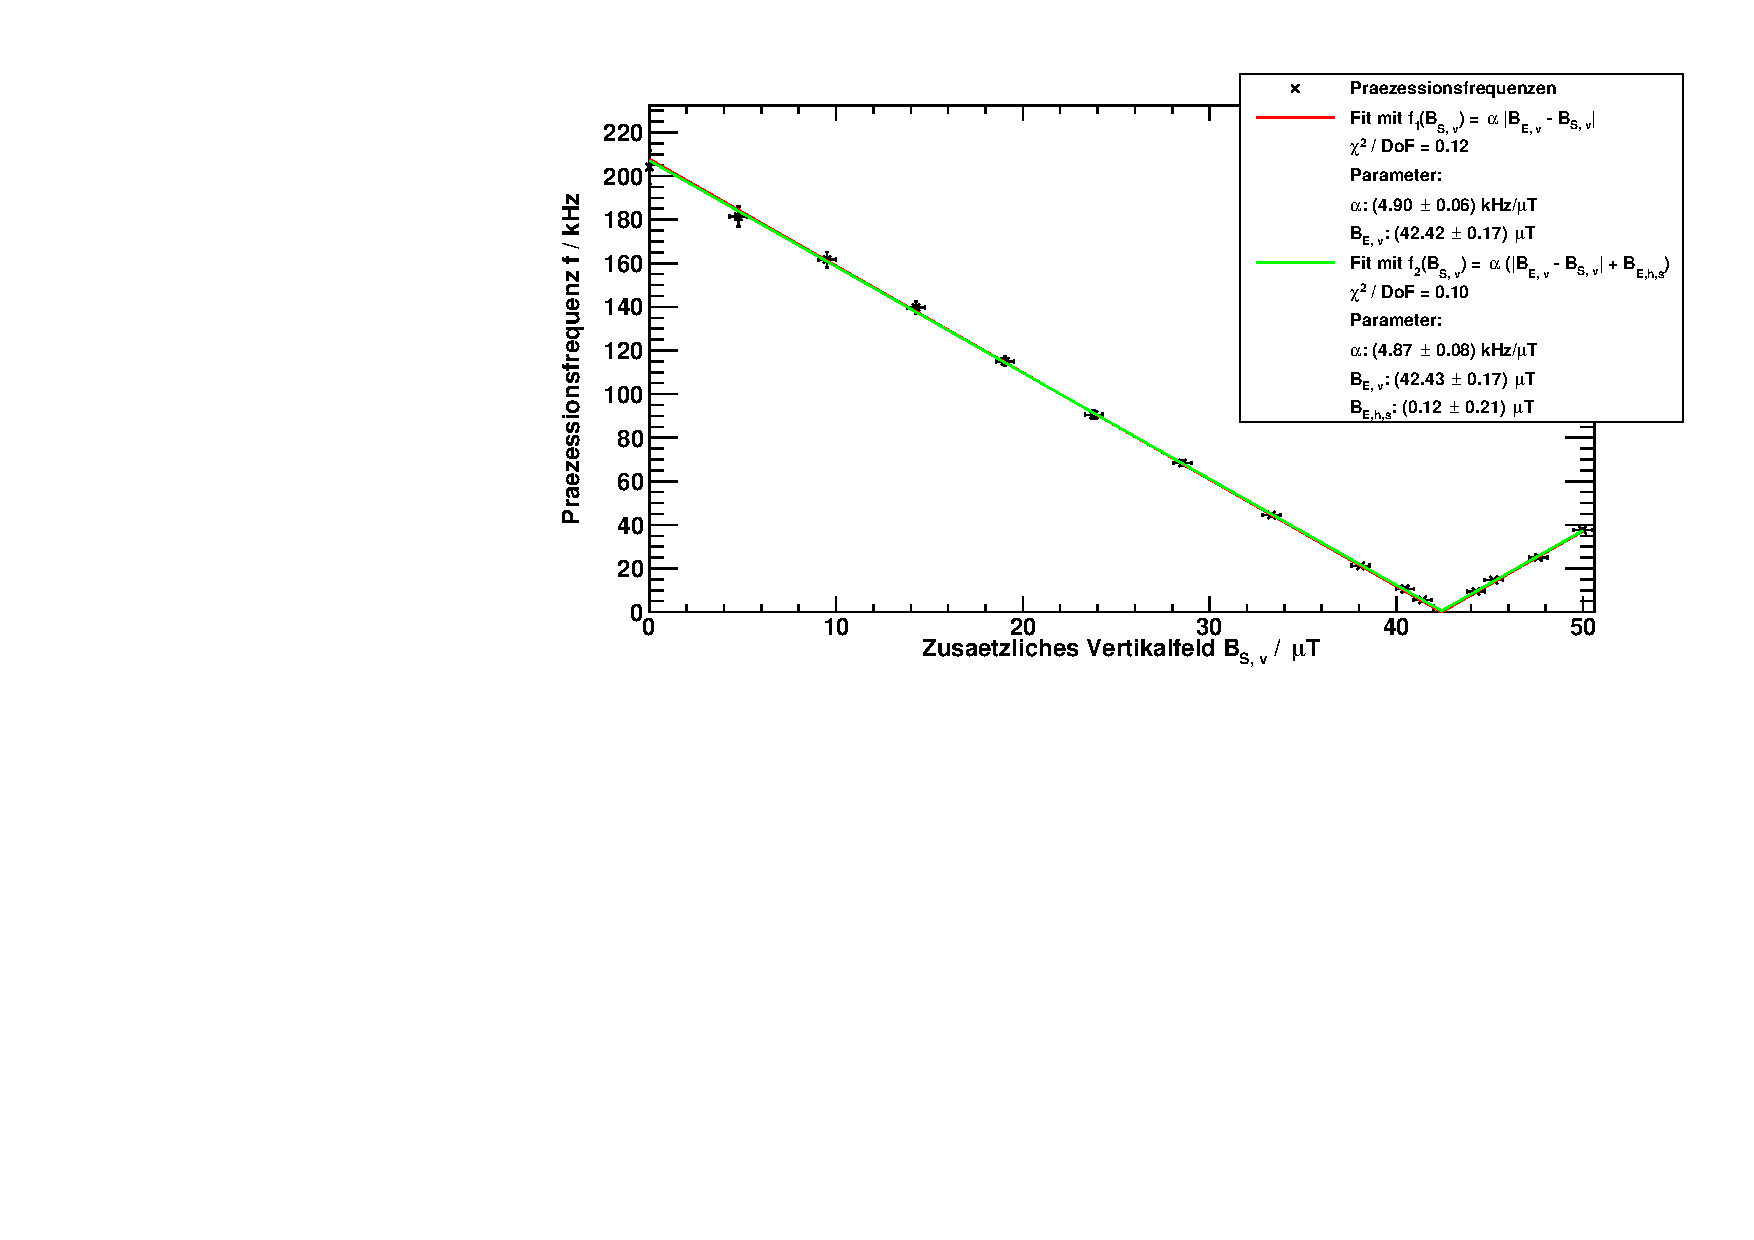
\includegraphics[width=\textwidth]{../img/part4/Rb85_gedreht.pdf}
  \caption{Spinpräzessionsfrequenz $f$ von \rb{85} in Abhängigkeit
  vom zusätzlichen vertikalen Magnetfeld $B_\text{S,v}$
  nach Drehung des Messaufbaus um 10$^\circ$ gegen den Uhrzeigersinn.}
  \label{img:spp:SPPRb87gedr}
\end{center}
\end{figure} 

Als Fitparameter erhält man
\begin{equation}
  B_\text{E,v} = (39.09\,\pm\,0.02)\,\text{\textmu T} \qquad \text{und} \qquad \alpha = (5.42\,\pm\,0.03)\,\text{ms}^{-1} \text{\textmu T}^{-1}
\end{equation}
Der Wert für das vertikale Erdmagnetfeld stimmt aus dem oben erwähnten Grund nicht mit dem Literaturwert überein.
Für die starke Abweichung des Parameters $\alpha$ vom theoretischen Wert $\alpha^\text{theo}$\,=\,4.665\,ms$^{-1}$\textmu T$^{-1}$ haben wir keine Erklärung.\\

Eine weitere Untersuchung der Horizontalkomponente erfolgte mit einer Untersuchung der Winkelabhängigkeit
der Präzessionsfrequenz.
Für sie gilt
\begin{equation}
  f(\varphi) = \alpha \cdot B_\text{E,h,p} \cdot |\sin(\varphi)| \ \, ,  %TODO Parameter für Winkeloffset, sollte verschwinden
\end{equation}
mit der Horizontalkomponente $B_\text{E,h,p}$ des Erdmagnetfelds in Strahlrichtung.
\autoref{img:spp:Winkelabhängigkeit} zeigt die Messergebnisse und den Fit mit obiger Gleichung.
Leider erlaubten die Abmessungen des Aufbaus eine Messung nur im Bereich von -10$^\circ$ bis 10$^\circ$,
so dass für den Sinus auch die Kleinwinkelnäherung verwendet werden könnte.

\begin{figure}[H]
\begin{center}
  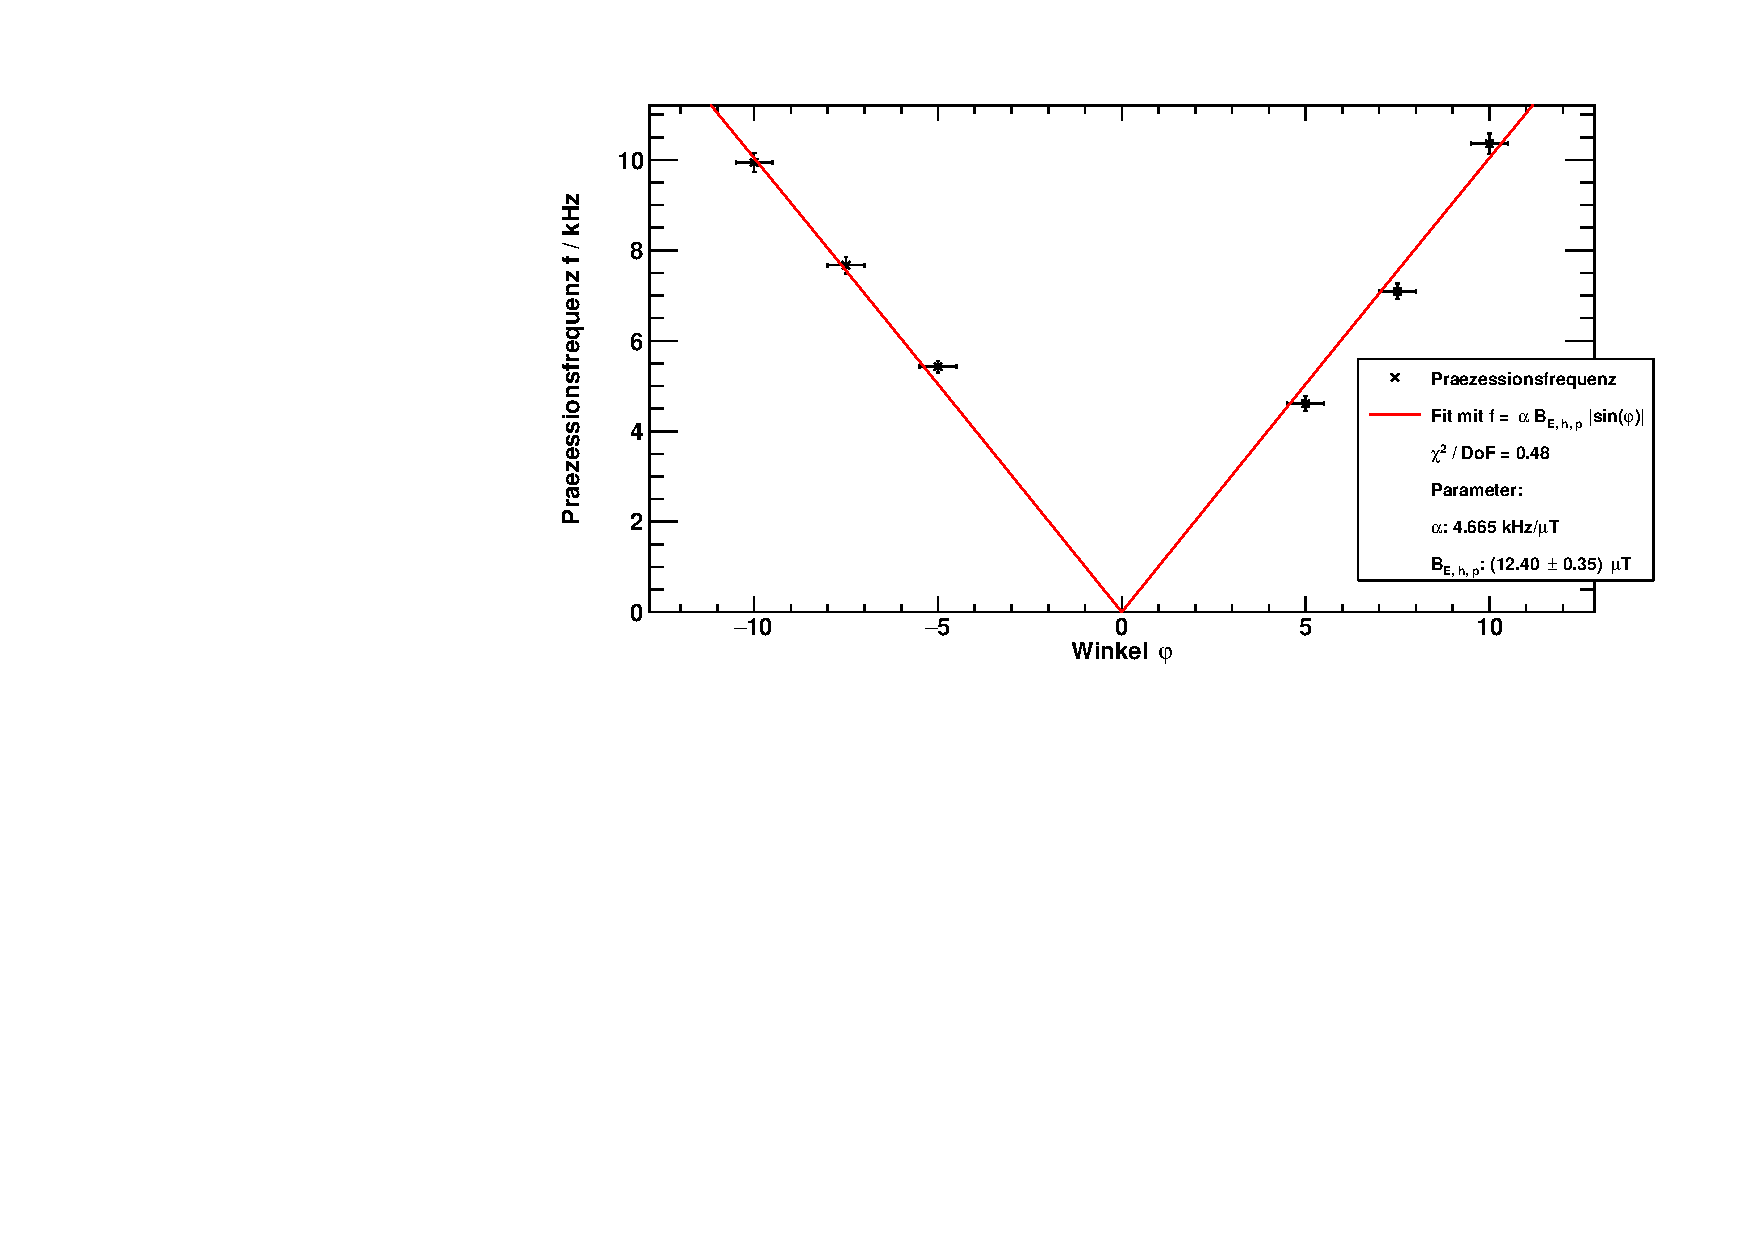
\includegraphics[width=\textwidth]{../img/part4/winkel.pdf}
  \caption{Abhängigkeit der Spinpräzessionsfrequenz $f$ von der Ausrichtung des Messaufbaus im Erdmagnetfeld.}
  \label{img:spp:Winkelabhängigkeit}
\end{center}
\end{figure} 

Die Horizontalkomponente des Erdmagnetfelds beträgt laut den oben gewonnenen Messdaten
\begin{equation}
  B_\text{E,h,p} = \sqrt{\bar{B}_\text{hor}^2+B_\text{E,h,s}^2}=(12.5 \pm 0.2)\,\text{\textmu T} \ \, .
\end{equation}
%TODO richtige Werte
Damit erhält man aus der Steigung der Fitgeraden $a$ für die Proportionalitätskonstante
\begin{equation}
  \alpha = \frac{a}{B_\text{E,h,p}} = (4.56\pm0.02)\,\text{ms}^{-1} \text{\textmu T}^{-1} \ \, .
\end{equation}
%TODO richtige Werte
Dieser Wert stimmt..
%TODO vgl Litval